\section{反三角函数}
\subsection{反三角函数的概念}
函数\(y = \sin x\ (-\frac\pi2 \leq x \leq \frac\pi2)\)的反函数,
叫做\DefineConcept{反正弦函数},
记作\(\arcsin x\).

函数\(y = \cos x\ (0 \leq x \leq \pi)\)的反函数,
叫做\DefineConcept{反余弦函数},
记作\(\arccos x\).

函数\(y = \tan x\ (-\frac\pi2 < x < \frac\pi2)\)的反函数,
叫做\DefineConcept{反正切函数},
记作\(\arctan x\).

正弦函数、余弦函数、正切函数、余切函数等三角函数的反函数,统称为\DefineConcept{反三角函数}.

\begin{figure}[htb]
	\centering
	\begin{tikzpicture}[scale=.5]
		\begin{axis}[
			xmin=-2,xmax=2,
			ymin=-2,ymax=2,
			grid=both,width=\textwidth,height=\textwidth,
			axis lines=middle,
			xlabel=$x$,
			ylabel=$y$,
			enlarge x limits=0.1,
			enlarge y limits=0.1,
			x label style={at={(ticklabel* cs:1.00)}, inner sep=5pt, anchor=west},
			y label style={at={(ticklabel* cs:1.00)}, inner sep=2pt, anchor=south},
			ytick={-1.5708,1.5708},
			yticklabels={
				$-\frac{\pi}{2}$,
				$\frac{\pi}{2}$,
			},
			xtick={-1,1},
			xticklabels={
				$-1$,
				$1$,
			}
		]
			\addplot[color=blue,samples=50,smooth,domain=-1:1,variable=\x]{asin(\x)/180*pi};
		\end{axis}
	\end{tikzpicture}
	\caption{反正弦函数\(y=\arcsin x\)的图形}
	\label{figure:函数.反正弦函数的图形}
\end{figure}

\begin{figure}[htb]
	\centering
	\begin{tikzpicture}[scale=.5]
		\begin{axis}[
			xmin=-2,xmax=2,
			ymin=0,ymax=3.5,
			grid=both,width=\textwidth,height=\textwidth,
			axis lines=middle,
			xlabel=$x$,
			ylabel=$y$,
			enlarge x limits=0.1,
			enlarge y limits=0.1,
			x label style={at={(ticklabel* cs:1.00)}, inner sep=5pt, anchor=west},
			y label style={at={(ticklabel* cs:1.00)}, inner sep=2pt, anchor=south},
			ytick={1.5708,3.1416},
			yticklabels={
				$\frac{\pi}{2}$,
				$\pi$,
			},
			xtick={-1,1},
		]
			\addplot[color=blue,samples=50,smooth,domain=-1:1,variable=\x]{acos(\x)/180*pi};
		\end{axis}
	\end{tikzpicture}
	\caption{反余弦函数\(y=\arccos x\)的图形}
	\label{figure:函数.反余弦函数的图形}
\end{figure}

\begin{figure}[htb]
	\centering
	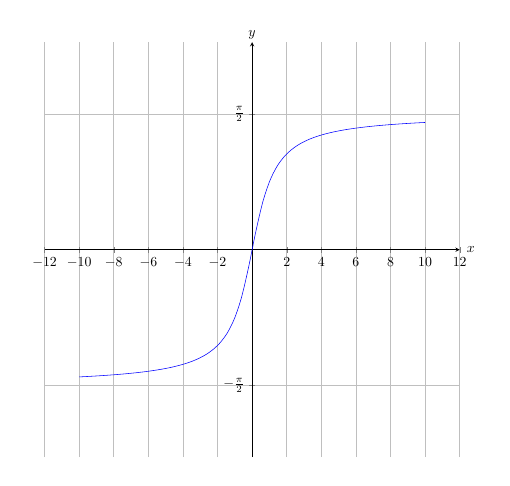
\begin{tikzpicture}[scale=.5]
		\begin{axis}[
			xmin=-10,xmax=10,
			ymin=-2,ymax=2,
			grid=both,width=\textwidth,height=\textwidth,
			axis lines=middle,
			xlabel=$x$,
			ylabel=$y$,
			enlarge x limits=0.1,
			enlarge y limits=0.1,
			x label style={at={(ticklabel* cs:1.00)}, inner sep=5pt, anchor=west},
			y label style={at={(ticklabel* cs:1.00)}, inner sep=2pt, anchor=south},
			ytick={-1.5708,1.5708},
			yticklabels={
				$-\frac{\pi}{2}$,
				$\frac{\pi}{2}$,
			},
		]
			\addplot[color=blue,samples=50,smooth,domain=-10:10,variable=\x]{atan(\x)/180*pi};
		\end{axis}
	\end{tikzpicture}
	\caption{反正切函数\(y=\arctan x\)的图形}
	\label{figure:函数.反正切函数的图形}
\end{figure}

\begin{figure}[htb]
	\centering
	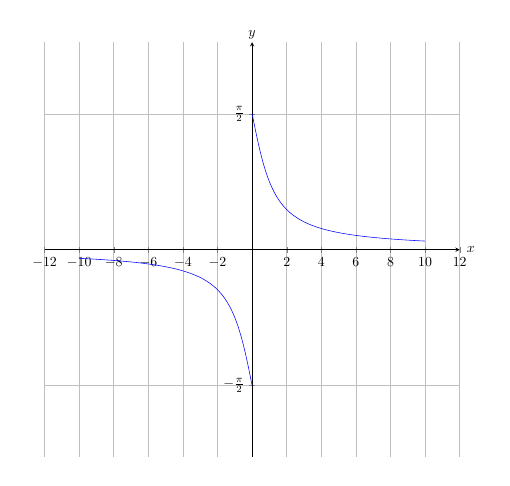
\begin{tikzpicture}[scale=.5]
		\begin{axis}[
			xmin=-10,xmax=10,
			ymin=-2,ymax=2,
			grid=both,width=\textwidth,height=\textwidth,
			axis lines=middle,
			xlabel=$x$,
			ylabel=$y$,
			enlarge x limits=0.1,
			enlarge y limits=0.1,
			x label style={at={(ticklabel* cs:1.00)}, inner sep=5pt, anchor=west},
			y label style={at={(ticklabel* cs:1.00)}, inner sep=2pt, anchor=south},
			ytick={-1.5708,1.5708},
			yticklabels={
				$-\frac{\pi}{2}$,
				$\frac{\pi}{2}$,
			},
		]
			\addplot[color=blue,samples=50,smooth,domain=0:10,variable=\x]{pi/2-atan(\x)/180*pi};
			\addplot[color=blue,samples=50,smooth,domain=-10:0,variable=\x]{-pi/2-atan(\x)/180*pi};
		\end{axis}
	\end{tikzpicture}
	\caption{反余切函数\(y=\arccot x\)的图形}
\end{figure}

\begin{figure}[htb]
	\centering
	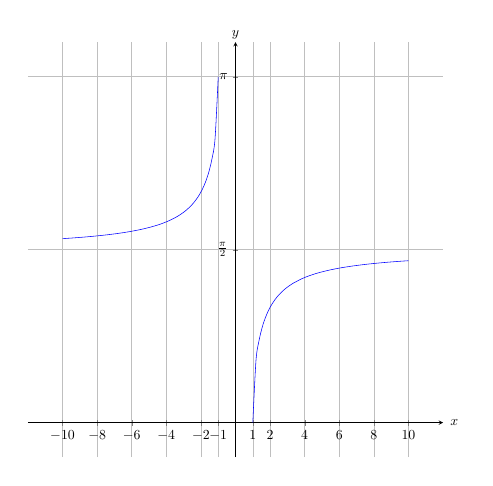
\begin{tikzpicture}[scale=.5]
		\begin{axis}[
			xmin=-10,xmax=10,
			ymin=0,ymax=pi,
			grid=both,width=\textwidth,height=\textwidth,
			axis lines=middle,
			xlabel=$x$,
			ylabel=$y$,
			enlarge x limits=0.1,
			enlarge y limits=0.1,
			x label style={at={(ticklabel* cs:1.00)}, inner sep=5pt, anchor=west},
			y label style={at={(ticklabel* cs:1.00)}, inner sep=2pt, anchor=south},
			xtick={-10,-8,...,-2,-1,1,2,4,...,10},
			ytick={1.5708,3.1416},
			yticklabels={
				$\frac{\pi}{2}$,
				$\pi$,
			},
		]
			\addplot[color=blue,samples=50,smooth,domain=1:10,variable=\x]{acos(1/\x)/180*pi};
			\addplot[color=blue,samples=50,smooth,domain=-10:-1,variable=\x]{acos(1/\x)/180*pi};
		\end{axis}
	\end{tikzpicture}
	\caption{反正割函数\(y=\arcsec x\)的图形}
\end{figure}

\begin{figure}[htb]
	\centering
	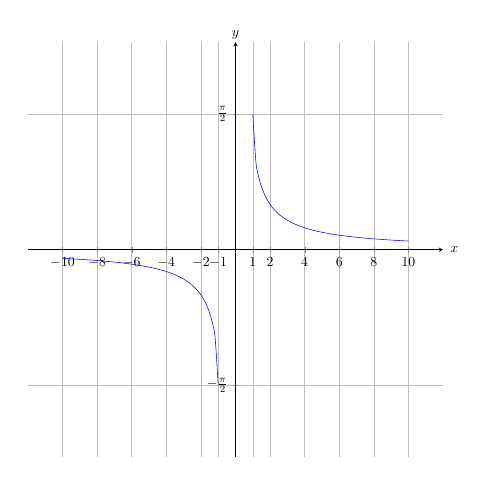
\begin{tikzpicture}[scale=.5]
		\begin{axis}[
			xmin=-10,xmax=10,
			ymin=-2,ymax=2,
			grid=both,width=\textwidth,height=\textwidth,
			axis lines=middle,
			xlabel=$x$,
			ylabel=$y$,
			enlarge x limits=0.1,
			enlarge y limits=0.1,
			x label style={at={(ticklabel* cs:1.00)}, inner sep=5pt, anchor=west},
			y label style={at={(ticklabel* cs:1.00)}, inner sep=2pt, anchor=south},
			xtick={-10,-8,...,-2,-1,1,2,4,...,10},
			ytick={-1.5708,1.5708},
			yticklabels={
				$-\frac{\pi}{2}$,
				$\frac{\pi}{2}$,
			},
		]
			\addplot[color=blue,samples=50,smooth,domain=1:10,variable=\x]{asin(1/\x)/180*pi};
			\addplot[color=blue,samples=50,smooth,domain=-10:-1,variable=\x]{asin(1/\x)/180*pi};
		\end{axis}
	\end{tikzpicture}
	\caption{反余割函数\(y=\arccsc x\)的图形}
\end{figure}

\subsection{反三角函数的性质}
反正弦函数\(y = \arcsin x\)的定义域是\([-1,1]\),
值域是\(\left[-\frac\pi2,\frac\pi2\right]\).

反余弦函数\(y = \arccos x\)的定义域是\([-1,1]\),
值域是\([0,\pi]\).

反正切函数\(y = \arctan x\)的定义域是\((-\infty,+\infty)\),
值域是\(\left(-\frac\pi2,\frac\pi2\right)\).

\begin{theorem}[余角公式]
\begin{gather}
	\arcsin x + \arccos x = \frac{\pi}{2}, \\
	\arctan x + \arccot x = \left\{ \def\arraystretch{1.5} \begin{array}{rl}
		\frac{\pi}{2}, & x > 0, \\
		-\frac{\pi}{2}, & x < 0.
	\end{array} \right.
\end{gather}
\end{theorem}

\begin{theorem}[负数关系]
\begin{gather}
	\arcsin(-x) = -\arcsin x, \\
	\arccos(-x) = \pi-\arccos x, \\
	\arctan(-x) = -\arctan x, \\
	\arccot(-x) = \pi-\arccot x, \\
	\arcsec(-x) = \pi-\arcsec x, \\
	\arccsc(-x) = -\arccsc x.
\end{gather}
\end{theorem}

\begin{theorem}[倒数关系]
\begin{gather}
	\arcsin\frac{1}{x} = \arccsc x, \\
	\arccos\frac{1}{x} = \arcsec x, \\
	\arctan\frac{1}{x} = \arccot x
		= \frac{\pi}{2} - \arctan x
	\quad(x>0), \\
	\arccot\frac{1}{x} = \left\{ \begin{array}{rl}
		\arctan x, & x>0, \\
		\pi+\arctan x, & x<0,
	\end{array} \right. \\
	\arccot\frac{1}{x} = \left\{ \def\arraystretch{2} \begin{array}{rc}
		\dfrac{\pi}{2} - \arccot x, & x>0, \\
		\dfrac{3\pi}{2} - \arccot x, & x<0,
		\end{array} \right. \\
	\arcsec\frac{1}{x} = \arccos x, \\
	\arccsc\frac{1}{x} = \arcsin x.
\end{gather}
\end{theorem}

\begin{theorem}[三角关系]
\begin{gather}
	\sin(\arcsin{x}) = x, \\
	\cos(\arccos{x}) = x, \\
	\tan(\arctan{x}) = x, \\
	\arcsin(\sin x) = x, \quad x \in (-\frac{\pi}{2},\frac{\pi}{2}), \\
	\arccos(\cos x) = x, \quad x \in (0,\pi), \\
	\arctan(\tan x) = x, \quad x \in (-\frac{\pi}{2},\frac{\pi}{2}), \\
	\sin(\arccos{x}) = \cos(\arcsin{x}) = \sqrt{1 - x^2}, \\
	\tan(\arccot{x}) = \cot(\arccot{x}) = \frac{1}{x}, \\
	\sin(\arctan{x}) = \cos(\arccot{x}) = \frac{x}{\sqrt{1+x^2}}, \\
	\cos(\arctan{x}) = \sin(\arccot{x}) = \frac{1}{\sqrt{1+x^2}}.
\end{gather}
\end{theorem}

\begin{theorem}[和差公式]
\begin{align}
	&\hspace{-10pt}
	\arcsin x + \arcsin y \notag \\
		&= \arcsin(x \sqrt{1-y^2} + y \sqrt{1-x^2})
			\quad(xy\leq0 \lor x^2+y^2\leq1) \\
		&= \pi - \arcsin(x \sqrt{1-y^2} + y \sqrt{1-x^2})
			\quad(x>0, y>0, x^2+y^2>1) \\
		&= -\pi - \arcsin(x \sqrt{1-y^2} + y \sqrt{1-x^2})
			\quad(x<0, y<0, x^2+y^2>1), \\
	&\hspace{-10pt}
	\arcsin x - \arcsin y \notag \\
		&= \arcsin(x \sqrt{1-y^2} - y \sqrt{1-x^2})
			\quad(xy\geq0 \lor x^2+y^2\leq1) \\
		&= \pi - \arcsin(x \sqrt{1-y^2} - y \sqrt{1-x^2})
			\quad(x>0, y<0, x^2+y^2>1) \\
		&= -\pi - \arcsin(x \sqrt{1-y^2} + y \sqrt{1-x^2})
			\quad(x<0, y>0, x^2+y^2>1), \\
	&\hspace{-10pt}
	\arccos x + \arccos y \notag \\
		&= \arccos[xy - \sqrt{(1-x^2)(1-y^2)}]
			\quad(x+y\geq0) \\
		&= 2\pi - \arccos[xy - \sqrt{(1-x^2)(1-y^2)}]
			\quad(x+y<0), \\
	&\hspace{-10pt}
	\arccos x - \arccos y \notag \\
		&= -\arccos[xy + \sqrt{(1-x^2)(1-y^2)}]
			\quad(x \geq y) \\
		&= \arccos[xy + \sqrt{(1-x^2)(1-y^2)}]
			\quad(x<y), \\
	&\hspace{-10pt}
	\arctan x + \arctan y \notag \\
		&= \arctan\frac{x+y}{1-xy}
			\quad(xy<1) \\
		&= \pi+\arctan\frac{x+y}{1-xy}
			\quad(x>0,xy>1) \\
		&= -\pi+\arctan\frac{x+y}{1-xy}
			\quad(x<0,xy>1), \\
	&\hspace{-10pt}
	\arctan x - \arctan y \notag \\
		&= \arctan\frac{x-y}{1+xy}
			\quad(xy>-1) \\
		&= \pi+\arctan\frac{x-y}{1+xy}
			\quad(x>0,xy<-1) \\
		&= -\pi+\arctan\frac{x-y}{1+xy}
			\quad(x<0,xy<-1).
\end{align}
\end{theorem}

\begin{figure}[htb]
	\centering
	\begin{tikzpicture}
		\draw[help lines, color=gray!30, dashed](0,0)grid(4,3);
		\coordinate(A)at(0,0);
		\coordinate(B)at(4,0);
		\coordinate(C)at(4,3);
		\draw (A)node[left]{\(A\)}
			--(B)node[right]{\(B\)}node[midway,below]{\(1\)}
			--(C)node[right]{\(C\)}node[midway,right]{\(x\)}
			--(A)node[midway,above left]{\(\sqrt{1+x^2}\)}
			pic["\(\theta\)",draw=orange,-,angle eccentricity=2,angle radius=0.3cm]{angle=B--A--C}
			pic[draw=gray,-,angle radius=0.3cm]{right angle=C--B--A};
		\draw (5,1.5)node[right]{\(\begin{aligned}
			&\tan\theta = x \implies \theta = \arctan x, \\
			&\cos\theta = \cos(\arctan x) = \frac{1}{\sqrt{1+x^2}}, \\
			&\sin\theta = \sin(\arctan x) = \frac{x}{\sqrt{1+x^2}}, \\
			&\cot\theta = \cot(\arctan x) = \frac{1}{x}.
		\end{aligned}\)};
	\end{tikzpicture}
	\caption{三角函数与反三角函数之间的联系}
\end{figure}
